\subsubsection{Planificación inicial} \label{sec:5-Planificacion-inicial}
\hypertarget{sec:5-Planificacion-inicial}{}
A partir de las tareas definidas en la sección \coloredUnderline{\hyperlink{sec:5-WBS}{\ref*{sec:5-WBS} \nameref*{sec:5-WBS}}} se ha realizado una planificación inicial del proyecto, en la que se han establecido las fechas de inicio y fin de cada tarea, así como su duración y las dependencias entre ellas. 
La planificación inicial se ha realizado en la herramienta \coloredUnderline{\href{https://www.microsoft.com/es-es/microsoft-365/p/project-profesional-2019/cfq7ttc0k7cj}{Microsoft Project}}.
Al igual que en la sección anterior, se ha dividido la planificación en las fases en las que se divide el proyecto para mejorar la legibilidad mostrando primero una visión general y después entrando en detalle en cada una de las fases.
Se incluye una tabla con las siguientes columnas:
\begin{itemize}
    \item \textbf{EDT:} Estructura de Desglose del Trabajo, también conocida como WBS. Detalla el identificador de la tarea.
    \item \textbf{Nombre tarea:} Nombre de la tarea.
    \item \textbf{Duración:} Duración de la tarea en horas.
    \item \textbf{Fecha inicio:} Fecha de inicio de la tarea.
    \item \textbf{Fecha fin:} Fecha de fin de la tarea.
\end{itemize}

Además, se incluye una línea temporal del proyecto para visualizar de forma más clara la planificación del proyecto así como el diagrama de Gantt de cada una de las fases del proyecto.

\subsubsubsection{Planificación inicial. Visión general}
En la \coloredUnderline{\hyperlink{table:5_PI-Vision-General}{\ref*{table:5_PI-Vision-General}: \nameref*{table:5_PI-Vision-General}}} se muestra la planificación inicial del proyecto de alto nivel, es decir, las tareas generales o fases que se deben realizar para cumplir con los objetivos del proyecto.
El total de días estimados para la realización del proyecto es de 71,13 días (462 horas), desde el 01/04/2024 hasta el 18/06/2024.


\begin{table}[H]
    \centering
    \caption{Planificación inicial. Visión general}
    \label{table:5_PI-Vision-General}
    \hypertarget{table:5_PI-Vision-General}{}
    \begin{tabular}{
       >{\columncolor{lightgreen!20}\raggedright\arraybackslash}p{1.5cm}
       >{\raggedright\arraybackslash}p{4.5cm}
       >{\raggedright\arraybackslash}p{2cm}
       >{\raggedright\arraybackslash}p{3cm}
       >{\raggedright\arraybackslash}p{3cm} }
    \rowcolor{darkgreen!50}
    \toprule
    \textbf{EDT} & \textbf{Nombre tarea} & \textbf{Duración} & \textbf{Fecha inicio} & \textbf{Fecha fin} \\
    \midrule
    1 & Proyecto BidMon Universe & 462 horas & 01/04/2024 & 18/06/2024 \\
    \midrule
    1.1 & Análisis del proyecto & 12 horas & 01/04/2024 & 12/04/2024 \\
    \midrule
    1.2 & Seguimiento del proyecto & 30,5 horas & 01/04/2024 & 18/06/2024 \\
    \midrule
    1.3 & Diseño del sistema & 76 horas & 03/04/2024 & 15/05/2024 \\
    \midrule
    1.4 & Implementación del sistema &  156,5 horas & 03/04/2024 & 22/05/2024 \\
    \midrule
    1.5 & Fase de pruebas & 9 horas & 28/05/2024 & 01/06/2024 \\
    \midrule
    1.6 & Despliegue del sistema & 8 horas & 12/06/2024 & 13/06/2024 \\
    \midrule
    1.7 & Documentación del proyecto & 170 horas & 02/04/2024 & 18/06/2024 \\
    \bottomrule
    \end{tabular}
\end{table}



En la \coloredUnderline{\hyperlink{fig:5_PI-Linea-Temporal}{Figura \ref*{fig:5_PI-Linea-Temporal}: \nameref*{fig:5_PI-Linea-Temporal}}} se muestra la línea temporal del proyecto.
Mediante esta planificación se pretende priorizar las tareas de análisis y diseño del sistema, para posteriormente realizar la implementación y las pruebas del sistema, y finalmente desplegar el sistema. 
La fase de documentación del proyecto se realizará de forma paralela a las demás tareas al igual que el seguimiento del proyecto.
\begin{figure}[H]
    \hypertarget{fig:5_PI-Linea-Temporal}{}
    \centering
    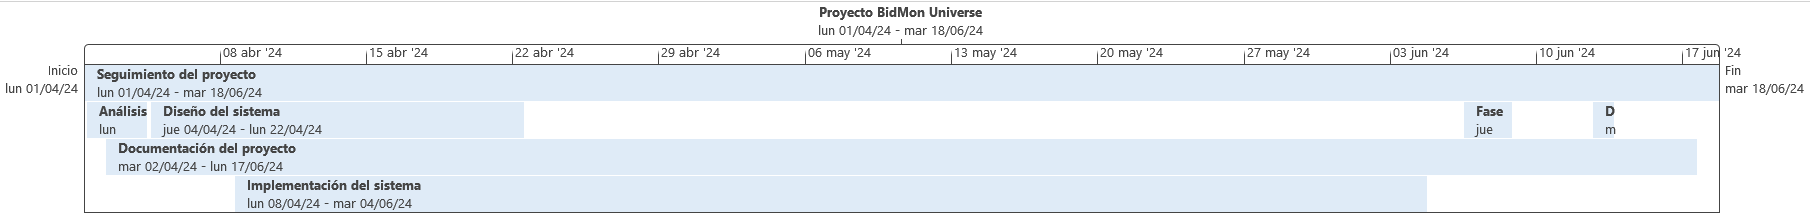
\includegraphics[width=1\linewidth]{figures/5_PI-Linea-Temporal.png}
    \caption{Planificación inicial. Línea temporal}
    \label{fig:5_PI-Linea-Temporal}
\end{figure}

En la \coloredUnderline{\hyperlink{fig:5_PI-Gantt}{Figura \ref*{fig:5_PI-Gantt}: \nameref*{fig:5_PI-Gantt}}} se muestra el diagrama de Gantt de la planificación inicial del proyecto.
\begin{figure}[H]
    \hypertarget{fig:5_PI-Gantt}{}
    \centering
    \includegraphics[width=1\linewidth]{figures/5-Gantt/5-Gantt-Vision-General.png}
    \caption{Planificación inicial. Diagrama de Gantt, visión general}
    \label{fig:5_PI-Gantt}
\end{figure}


\subsubsubsection{Planificación inicial. Análisis del proyecto}
En la \coloredUnderline{\hyperlink{table:5_PI-Analisis}{\ref*{table:5_PI-Analisis}: \nameref*{table:5_PI-Analisis}}}, se detallan la planificación de las tareas que se deben realizar en la fase de análisis del sistema.
El total de horas estimadas para la realización de esta fase es de 12 horas, desde el 01/04/2024 hasta el 12/04/2024.
\begin{table}[H]
    \centering
    \caption{Planificación inicial. Análisis del proyecto}
    \label{table:5_PI-Analisis}
    \hypertarget{table:5_PI-Analisis}{}
    \begin{tabular}{
       >{\columncolor{lightgreen!20}\raggedright\arraybackslash}p{1.5cm}
       >{\raggedright\arraybackslash}p{4.5cm}
       >{\raggedright\arraybackslash}p{2cm}
       >{\raggedright\arraybackslash}p{3cm}
       >{\raggedright\arraybackslash}p{3cm} }
    \rowcolor{darkgreen!50}
    \toprule
    \textbf{EDT} & \textbf{Nombre tarea} & \textbf{Duración} & \textbf{Fecha inicio} & \textbf{Fecha fin} \\
    \midrule
    1.1 & Análisis del proyecto & 12 horas & 01/04/2024 & 12/04/2024 \\
    \midrule
    1.1.1 & Análisis del sistema & 5 horas & 01/04/2024 & 02/04/2024 \\
    \midrule
    1.1.2 & Análisis de la arquitectura & 3 horas & 11/04/2024 & 11/04/2024 \\
    \midrule
    1.1.3 & Análisis de la infraestructura & 4 horas & 12/04/2024 & 12/04/2024 \\
    \midrule
    1.1.4 & Determinación del análisis & 2 horas & 12/04/2024 & 12/04/2024 \\
    \bottomrule
    \end{tabular}
\end{table}

En la \coloredUnderline{\hyperlink{fig:5_PI-Gantt-Analisis}{Figura \ref*{fig:5_PI-Gantt-Analisis}: \nameref*{fig:5_PI-Gantt-Analisis}}}, se muestra el diagrama de Gantt de la planificación inicial de la fase de análisis del proyecto.
\begin{figure}[H]
    \hypertarget{fig:5_PI-Gantt-Analisis}{}
    \centering
    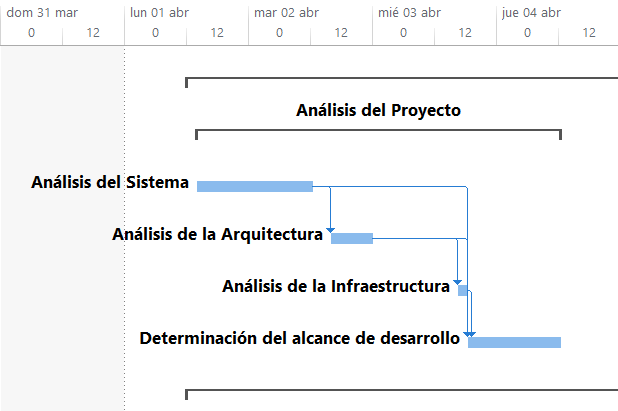
\includegraphics[width=1\linewidth]{figures/5-Gantt/5-Gantt-Analisis.png}
    \caption{Planificación inicial. Diagrama de Gantt, análisis del proyecto}
    \label{fig:5_PI-Gantt-Analisis}
\end{figure}



\subsubsubsection{Planificación inicial. Seguimiento del proyecto}
En la \coloredUnderline{\hyperlink{table:5_PI-Seguimiento}{\ref*{table:5_PI-Seguimiento}: \nameref*{table:5_PI-Seguimiento}}}, se detalla la planificación de las tareas que se deben realizar en la fase de seguimiento del proyecto.
El total de horas estimadas para la realización de esta fase es de 30,5 horas, desde el 01/04/2024 hasta el 18/06/2024, abarca todo el proyecto debido a que se realiza una reunión inicial, reuniones periódicas y una reunión final para la revisión del proyecto.
\begin{table}[H]
    \centering
    \caption{Planificación inicial. Seguimiento del proyecto}
    \label{table:5_PI-Seguimiento}
    \hypertarget{table:5_PI-Seguimiento}{}
    \begin{tabular}{
       >{\columncolor{lightgreen!20}\raggedright\arraybackslash}p{1.5cm}
       >{\raggedright\arraybackslash}p{4.5cm}
       >{\raggedright\arraybackslash}p{2cm}
       >{\raggedright\arraybackslash}p{3cm}
       >{\raggedright\arraybackslash}p{3cm} }
    \rowcolor{darkgreen!50}
    \toprule
    \textbf{EDT} & \textbf{Nombre tarea} & \textbf{Duración} & \textbf{Fecha inicio} & \textbf{Fecha fin} \\
    \midrule
    1.2 & Seguimiento del proyecto & 30,5 horas & 01/04/2024 & 12/04/2024 \\
    \midrule
    1.2.1 & Reunión de arranque & 2 horas & 01/04/2024 & 01/04/2024 \\
    \midrule
    1.2.2 & Reuniones periódicas & 20,5 horas & 27/04/2024 & 30/04/2024 \\
    \midrule
    1.2.3 & Reunión de revisión & 4 horas & 15/06/2024 & 15/06/2024 \\
    \midrule
    1.2.4 & Reunión final & 4 horas & 17/04/2024 & 18/04/2024 \\
    \bottomrule
    \end{tabular}
\end{table}

En la \coloredUnderline{\hyperlink{fig:5_PI-Gantt-Seguimiento}{Figura \ref*{fig:5_PI-Gantt-Seguimiento}: \nameref*{fig:5_PI-Gantt-Seguimiento}}}, se muestra el diagrama de Gantt de la planificación inicial de la fase de seguimiento del proyecto.
\begin{figure}[H]
    \hypertarget{fig:5_PI-Gantt-Seguimiento}{}
    \centering
    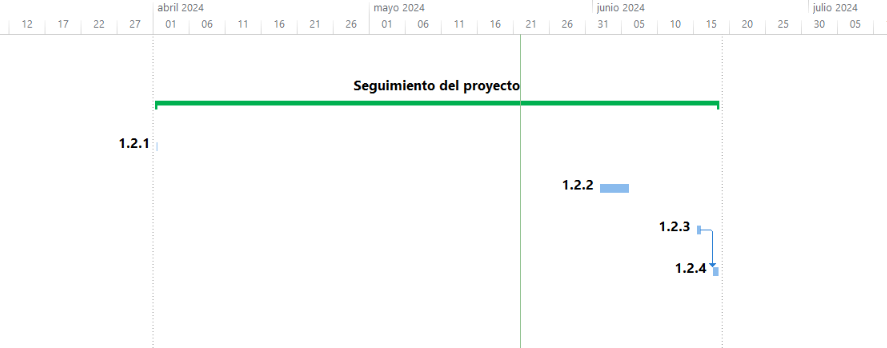
\includegraphics[width=1\linewidth]{figures/5-Gantt/5-Gantt-Seguimiento.png}
    \caption{Planificación inicial. Diagrama de Gantt, seguimiento del proyecto}
    \label{fig:5_PI-Gantt-Seguimiento}
\end{figure}



\subsubsubsection{Planificación inicial. Diseño del sistema}
En la \coloredUnderline{\hyperlink{table:5_PI-Diseno}{\ref*{table:5_PI-Diseno}: \nameref*{table:5_PI-Diseno}}}, se detalla la planificación de las tareas que se deben realizar en la fase de diseño del sistema.
El total de horas estimadas para la realización de esta fase es de 76 horas, desde el 03/04/2024 hasta el 15/05/2024.
\begin{longtable}{
    >{\columncolor{lightgreen!20}\raggedright\arraybackslash}p{1.5cm}
    >{\raggedright\arraybackslash}p{4.5cm}
    >{\raggedright\arraybackslash}p{2cm}
    >{\raggedright\arraybackslash}p{3cm}
    >{\raggedright\arraybackslash}p{3cm} }
    \caption{Planificación inicial. Diseño del sistema} \label{table:5_PI-Diseno} 
    \hypertarget{table:5_PI-Diseno}{}
    \\

    \toprule
    \rowcolor{darkgreen!50}
    \textbf{EDT} & \textbf{Nombre tarea} & \textbf{Duración} & \textbf{Fecha inicio} & \textbf{Fecha fin} \\
    \midrule
    \endfirsthead

    \toprule
    \rowcolor{darkgreen!50}
    \textbf{EDT} & \textbf{Nombre tarea} & \textbf{Duración} & \textbf{Fecha inicio} & \textbf{Fecha fin} \\
    \midrule
    \endhead

    \midrule
    \multicolumn{5}{r}{{Continúa en la siguiente página\ldots}} \\
    \endfoot

    \bottomrule
    \endlastfoot

    
    1.3 & Diseño del sistema & 76 horas & 03/04/2024 & 15/05/2024 \\
    \midrule
    1.3.1 & Diseño del \textit{backend} & 22 horas & 03/04/2024 & 16/04/2024 \\
    \midrule
    1.3.1.1 & Diseño del módulo de usuarios & 2 horas & 08/04/2024 & 08/04/2024 \\
    \midrule
    1.3.1.2 & Diseño del módulo de cartas & 6 horas & 03/04/2024 & 03/04/2024 \\
    \midrule
    1.3.1.3 & Diseño del módulo de sobres de cartas & 3 horas & 06/04/2024 & 08/04/2024 \\
    \midrule
    1.3.1.4 & Diseño del módulo de subastas & 6.5 horas & 09/04/2024 & 10/04/2024 \\
    \midrule
    1.3.1.5 & Diseño del módulo de transacciones & 4.5 horas & 16/04/2024 & 16/04/2024 \\
    \midrule
    1.3.2 & Diseño del \textit{frontend} & 11.81 días & 13/04/2024 & 26/04/2024 \\
    \midrule
    1.3.2.1 & Diseño de elementos gráficos & 1.13 días & 13/04/2024 & 13/04/2024 \\
    \midrule
    1.3.2.1.1 & Diseño de la moneda de la aplicación & 1 hora & 13/04/2024 & 13/04/2024 \\
    \midrule
    1.3.2.1.2 & Diseño del logo de la aplicación & 2 horas & 13/04/2024 & 13/04/2024 \\
    \midrule
    1.3.2.2 & Diseño de la temática & 2 horas & 13/04/2024 & 13/04/2024 \\
    \midrule
    1.3.2.3 & Diseño del árbol de navegación & 2 horas & 13/04/2024 & 13/04/2024 \\
    \midrule
    1.3.2.4 & Diseño de la interfaz de usuario & 9.44 días & 15/04/2024 & 26/04/2024 \\
    \midrule
    1.3.2.4.1 & Diseño de las páginas de información & 3 horas & 24/04/2024 & 25/04/2024 \\
    \midrule
    1.3.2.4.2 & Diseño de la página Home & 4 horas & 23/04/2024 & 24/04/2024 \\
    \midrule
    1.3.2.4.3 & Diseño de la página de error & 1 hora & 25/04/2024 & 25/04/2024 \\
    \midrule
    1.3.2.4.4 & Diseño del módulo de usuarios & 5.5 horas & 22/04/2024 & 23/04/2024 \\
    \midrule
    1.3.2.4.5 & Diseño del módulo de cartas & 4 horas & 19/04/2024 & 19/04/2024 \\
    \midrule
    1.3.2.4.6 & Diseño del módulo de sobres de cartas & 2 horas & 24/04/2024 & 24/04/2024 \\
    \midrule
    1.3.2.4.7 & Diseño del módulo de subastas & 5.5 horas & 15/04/2024 & 15/04/2024 \\
    \midrule
    1.3.2.4.8 & Diseño del módulo de transacciones & 4 horas & 25/04/2024 & 26/04/2024 \\
    \midrule
    1.3.3 & Diseño de pruebas & 4.19 días & 11/05/2024 & 15/05/2024 \\
    \midrule
    1.3.3.1 & Diseño de pruebas unitarias & 6.5 horas & 11/05/2024 & 11/05/2024 \\
    \midrule
    1.3.3.2 & Diseño de pruebas de carga/estrés & 5 horas & 14/05/2024 & 15/05/2024 \\
    \midrule
    1.3.3.3 & Diseño de pruebas \textit{end-to-end} & 6.5 horas & 11/05/2024 & 13/05/2024 \\
    \bottomrule
    \end{longtable}

A continuación se muestra el diagrama de Gantt de la planificación inicial de la fase de diseño del sistema. Se ha dividido en tres partes para mejorar la legibilidad estas partes son: diseño del \textit{backend}, diseño del \textit{frontend} y diseño de pruebas.
En la \coloredUnderline{\hyperlink{fig:5_PI-Gantt-Diseno-1}{Figura \ref*{fig:5_PI-Gantt-Diseno-1}: \nameref*{fig:5_PI-Gantt-Diseno-1}}}, se muestra parte de la fase de diseño del sistema correspondiente con el \textit{backend}.
\begin{figure}[H]
    \hypertarget{fig:5_PI-Gantt-Diseno-1}{}
    \centering
    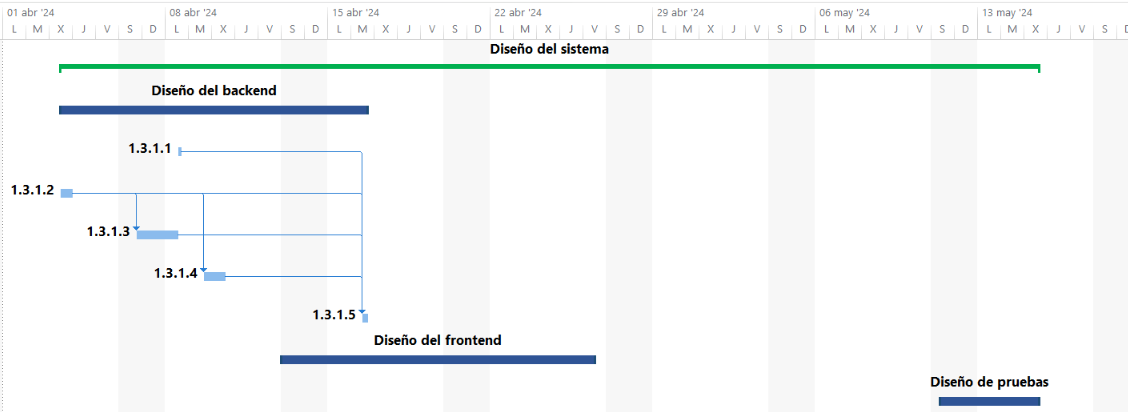
\includegraphics[width=1\linewidth]{figures/5-Gantt/5-Gantt-Diseno-backend.png}
    \caption{Planificación inicial. Diagrama de Gantt, diseño del sistema \textit{backend}}
    \label{fig:5_PI-Gantt-Diseno-1}
\end{figure}
En la \coloredUnderline{\hyperlink{fig:5_PI-Gantt-Diseno-2}{Figura \ref*{fig:5_PI-Gantt-Diseno-2}: \nameref*{fig:5_PI-Gantt-Diseno-2}}}, se muestra parte de la fase de diseño del sistema correspondiente con el \textit{frontend}.
\begin{figure}[H]
    \hypertarget{fig:5_PI-Gantt-Diseno-2}{}
    \centering
    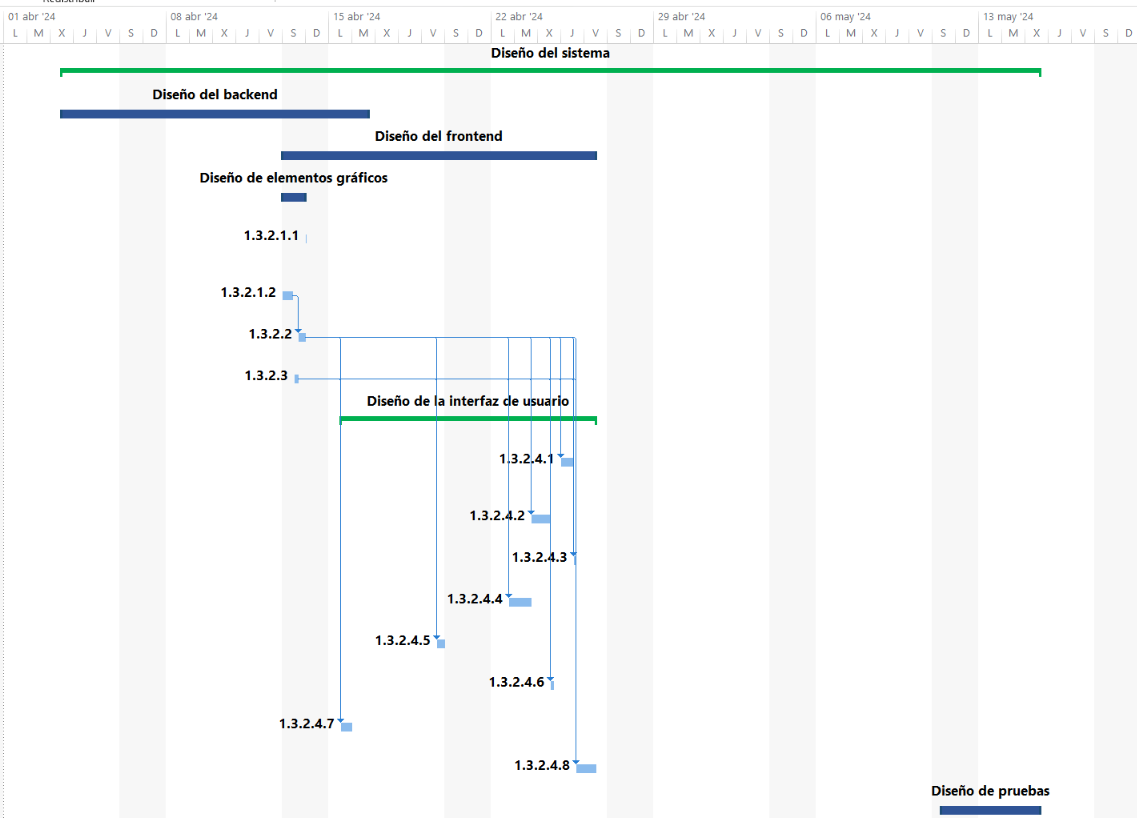
\includegraphics[width=1\linewidth]{figures/5-Gantt/5-Gantt-Diseno-frontend.png}
    \caption{Planificación inicial. Diagrama de Gantt, diseño del sistema \textit{frontend}}
    \label{fig:5_PI-Gantt-Diseno-2}
\end{figure}
En la \coloredUnderline{\hyperlink{fig:5_PI-Gantt-Diseno-3}{Figura \ref*{fig:5_PI-Gantt-Diseno-3}: \nameref*{fig:5_PI-Gantt-Diseno-3}}}, se muestra parte de la fase de diseño del sistema correspondiente con las pruebas.
\begin{figure}[H]
    \hypertarget{fig:5_PI-Gantt-Diseno-3}{}
    \centering
    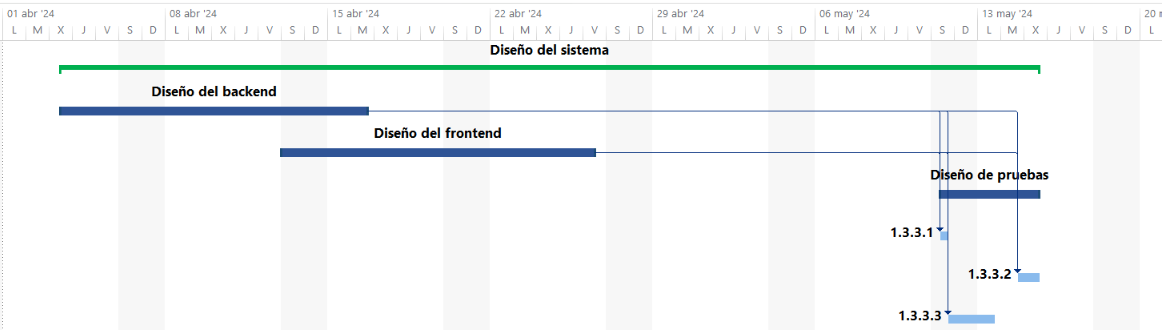
\includegraphics[width=1\linewidth]{figures/5-Gantt/5-Gantt-Diseno-pruebas.png}
    \caption{Planificación inicial. Diagrama de Gantt, diseño de pruebas}
    \label{fig:5_PI-Gantt-Diseno-3}
\end{figure}


\subsubsubsection{Planificación inicial. Implementación del sistema}
En la \coloredUnderline{\hyperlink{table:5_PI-Implementacion}{\ref*{table:5_PI-Implementacion}: \nameref*{table:5_PI-Implementacion}}}, se detalla la planificación de las tareas que se deben realizar en la fase de implementación del sistema.
El total de horas estimadas para la realización de esta fase es de 156,5 horas, desde el 03/04/2024 hasta el 22/05/2024.
\begin{longtable}{
    >{\columncolor{lightgreen!20}\raggedright\arraybackslash}p{1.5cm}
    >{\raggedright\arraybackslash}p{4.5cm}
    >{\raggedright\arraybackslash}p{2cm}
    >{\raggedright\arraybackslash}p{3cm}
    >{\raggedright\arraybackslash}p{3cm} }
    \caption{Planificación inicial. Implementación del sistema} \label{table:5_PI-Implementacion} 
    \hypertarget{table:5_PI-Implementacion}{}
    \\

    \toprule
    \rowcolor{darkgreen!50}
    \textbf{EDT} & \textbf{Nombre tarea} & \textbf{Duración} & \textbf{Fecha inicio} & \textbf{Fecha fin} \\
    \midrule
    \endfirsthead

    \toprule
    \rowcolor{darkgreen!50}
    \textbf{EDT} & \textbf{Nombre tarea} & \textbf{Duración} & \textbf{Fecha inicio} & \textbf{Fecha fin} \\
    \midrule
    \endhead

    \midrule
    \multicolumn{5}{r}{{Continúa en la siguiente página\ldots}} \\
    \endfoot

    \bottomrule
    \endlastfoot

    1.4 & Implementación del sistema & 43.44 días & 03/04/2024 & 22/05/2024 \\
    \midrule
    1.4.1 & Implementación del \textit{backend} & 39.13 días & 03/04/2024 & 17/05/2024 \\
    \midrule
    1.4.1.1 & Implementación del módulo de usuarios & 5.5 horas & 08/04/2024 & 09/04/2024 \\
    \midrule
    1.4.1.2 & Implementación del módulo de cartas & 20.5 horas & 03/04/2024 & 06/04/2024 \\
    \midrule
    1.4.1.3 & Implementación del módulo de sobres de cartas & 7.5 horas & 10/04/2024 & 11/04/2024 \\
    \midrule
    1.4.1.4 & Implementación del módulo de subastas & 17 horas & 16/04/2024 & 19/04/2024 \\
    \midrule
    1.4.1.5 & Implementación del módulo de transacciones & 16 horas & 15/05/2024 & 17/05/2024 \\
    \midrule
    1.4.2 & Implementación del \textit{frontend} & 26.38 días & 15/04/2024 & 14/05/2024 \\
    \midrule
    1.4.2.1 & Implementación de la temática & 1 hora & 15/04/2024 & 15/04/2024 \\
    \midrule
    1.4.2.2 & Implementación de las rutas de navegación & 1 hora & 01/05/2024 & 01/05/2024 \\
    \midrule
    1.4.2.3 & Implementación de la interfaz & 11.69 días & 01/05/2024 & 14/05/2024 \\
    \midrule
    1.4.2.3.1 & Implementación de las páginas de información & 3 horas & 01/05/2024 & 02/05/2024 \\
    \midrule
    1.4.2.3.2 & Implementación de la página Home & 8.5 horas & 02/05/2024 & 03/05/2024 \\
    \midrule
    1.4.2.3.3 & Implementación de la página de error & 1 hora & 01/05/2024 & 01/05/2024 \\
    \midrule
    1.4.2.3.4 & Implementación del módulo de usuarios & 8.5 horas & 03/05/2024 & 04/05/2024 \\
    \midrule
    1.4.2.3.5 & Implementación del módulo de cartas & 10.5 horas & 04/05/2024 & 07/05/2024 \\
    \midrule
    1.4.2.3.6 & Implementación del módulo de sobres de cartas & 7.5 horas & 07/05/2024 & 08/05/2024 \\
    \midrule
    1.4.2.3.7 & Implementación del módulo de subastas & 17 horas & 08/05/2024 & 11/05/2024 \\
    \midrule
    1.4.2.3.8 & Implementación del módulo de transacciones & 6.5 horas & 13/05/2024 & 14/05/2024 \\
    \midrule
    1.4.3 & Implementación de pruebas & 4.31 días & 18/05/2024 & 22/05/2024 \\
    \midrule
    1.4.3.1 & Implementación de pruebas unitarias & 13.5 horas & 18/05/2024 & 20/05/2024 \\
    \midrule
    1.4.3.2 & Implementación de pruebas de carga/estrés & 5.5 horas & 21/05/2024 & 22/05/2024 \\
    \midrule
    1.4.3.3 & Implementación de pruebas \textit{end-to-end} & 6.5 horas & 20/05/2024 & 21/05/2024 \\
    \end{longtable}

Al igual que en la fase de diseño del sistema, se ha dividido la fase de implementación en tres partes para mejorar la legibilidad estas partes son: implementación del \textit{backend}, implementación del \textit{frontend} e implementación de pruebas.
En la \coloredUnderline{\hyperlink{fig:5_PI-Gantt-Implementacion-1}{Figura \ref*{fig:5_PI-Gantt-Implementacion-1}: \nameref*{fig:5_PI-Gantt-Implementacion-1}}}, se muestra parte de la fase de implementación del sistema correspondiente con el \textit{backend}.
\begin{figure}[H]
    \hypertarget{fig:5_PI-Gantt-Implementacion-1}{}
    \centering
    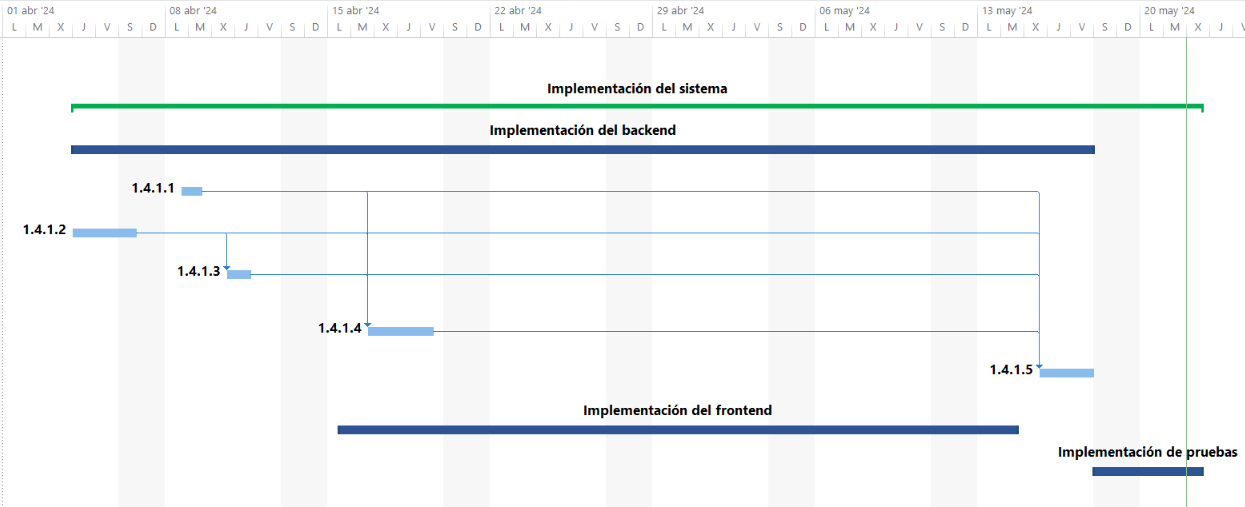
\includegraphics[width=1\linewidth]{figures/5-Gantt/5-Gantt-Implementacion-backend.png}
    \caption{Planificación inicial. Diagrama de Gantt, implementación del sistema \textit{backend}}
    \label{fig:5_PI-Gantt-Implementacion-1}
\end{figure}

En la \coloredUnderline{\hyperlink{fig:5_PI-Gantt-Implementacion-2}{Figura \ref*{fig:5_PI-Gantt-Implementacion-2}: \nameref*{fig:5_PI-Gantt-Implementacion-2}}}, se muestra parte de la fase de implementación del sistema correspondiente con el \textit{frontend}.
\begin{figure}[H]
    \hypertarget{fig:5_PI-Gantt-Implementacion-2}{}
    \centering
    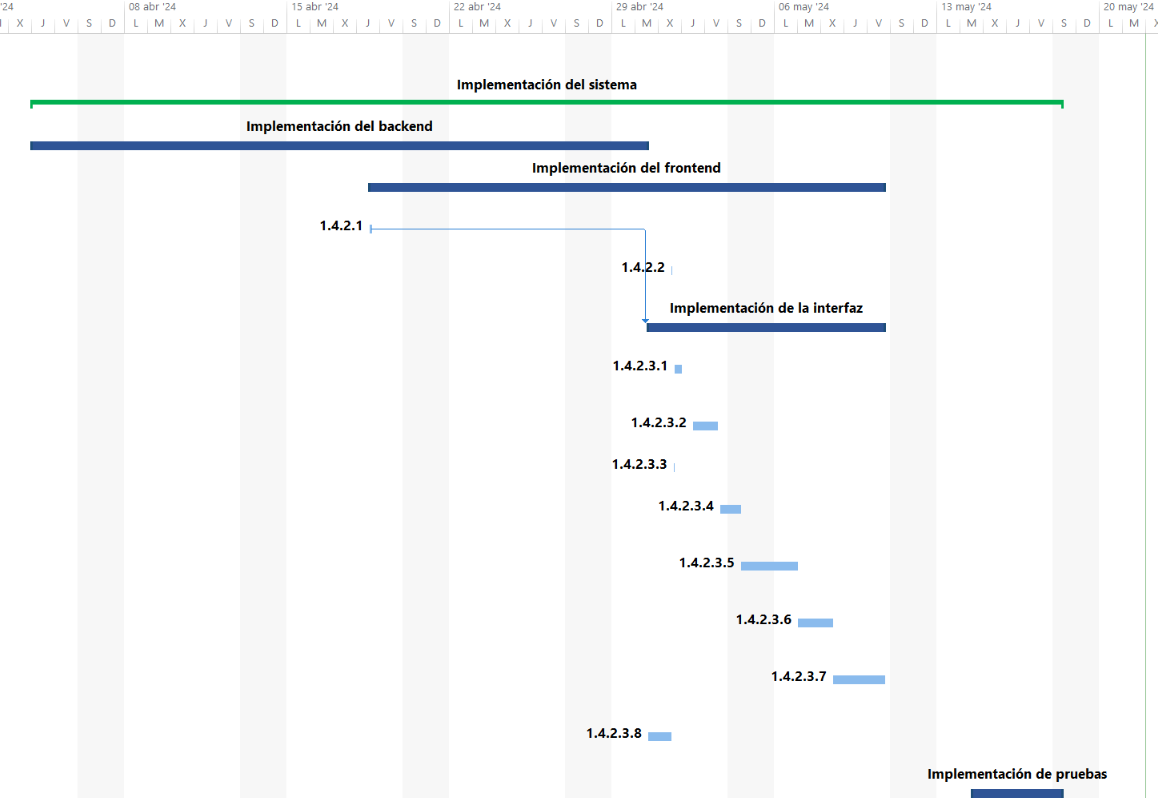
\includegraphics[width=1\linewidth]{figures/5-Gantt/5-Gantt-Implementacion-frontend.png}
    \caption{Planificación inicial. Diagrama de Gantt, implementación del sistema \textit{frontend}}
    \label{fig:5_PI-Gantt-Implementacion-2}
\end{figure}
Por último, en la \coloredUnderline{\hyperlink{fig:5_PI-Gantt-Implementacion-3}{Figura \ref*{fig:5_PI-Gantt-Implementacion-3}: \nameref*{fig:5_PI-Gantt-Implementacion-3}}}, se muestra parte de la fase de implementación del sistema correspondiente con las pruebas.
\begin{figure}[H]
    \hypertarget{fig:5_PI-Gantt-Implementacion-3}{}
    \centering
    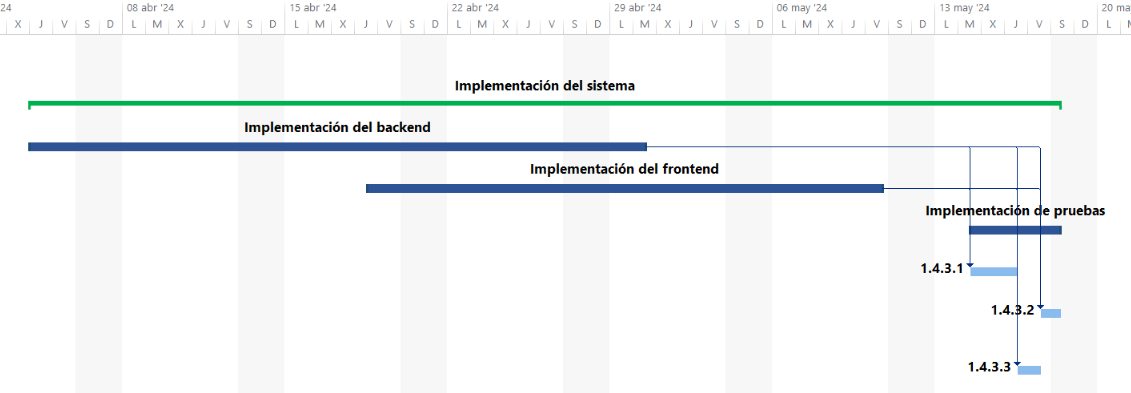
\includegraphics[width=1\linewidth]{figures/5-Gantt/5-Gantt-Implementacion-pruebas.png}
    \caption{Planificación inicial. Diagrama de Gantt, implementación de pruebas}
    \label{fig:5_PI-Gantt-Implementacion-3}
\end{figure}


\subsubsubsection{Planificación inicial. Fase de pruebas}
En la \coloredUnderline{\hyperlink{table:5_PI-Pruebas}{\ref*{table:5_PI-Pruebas}: \nameref*{table:5_PI-Pruebas}}}, se detalla la planificación de las tareas que se deben realizar en la fase de pruebas del sistema.
El total de horas estimadas para la realización de esta fase es de 9 horas, desde el 28/05/2024 hasta el 01/06/2024.
\begin{table}[H]
    \centering
    \caption{Planificación inicial. Fase de pruebas}
    \label{table:5_PI-Pruebas}
    \hypertarget{table:5_PI-Pruebas}{}
    \begin{tabular}{
       >{\columncolor{lightgreen!20}\raggedright\arraybackslash}p{1.5cm}
       >{\raggedright\arraybackslash}p{4.5cm}
       >{\raggedright\arraybackslash}p{2cm}
       >{\raggedright\arraybackslash}p{3cm}
       >{\raggedright\arraybackslash}p{3cm} }
    \rowcolor{darkgreen!50}
    \toprule
    \textbf{EDT} & \textbf{Nombre tarea} & \textbf{Duración} & \textbf{Fecha inicio} & \textbf{Fecha fin} \\
    \midrule
    1.5 & Fase de pruebas & 9 horas & 28/05/2024 & 01/06/2024 \\
    \midrule
    1.5.1 & Pruebas unitarias & 3 horas & 28/05/2024 & 29/05/2024 \\
    \midrule
    1.5.2 & Pruebas de carga/estrés & 3 horas & 31/05/2024 & 01/06/2024 \\
    \midrule
    1.5.3 & Pruebas \textit{end-to-end} & 3 horas & 29/05/2024 & 29/05/2024 \\
    \bottomrule
    \end{tabular}
\end{table}

En la \coloredUnderline{\hyperlink{fig:5_PI-Gantt-Pruebas}{Figura \ref*{fig:5_PI-Gantt-Pruebas}: \nameref*{fig:5_PI-Gantt-Pruebas}}}, se muestra el diagrama de Gantt de la planificación inicial de la fase de pruebas del sistema.
\begin{figure}[H]
    \hypertarget{fig:5_PI-Gantt-Pruebas}{}
    \centering
    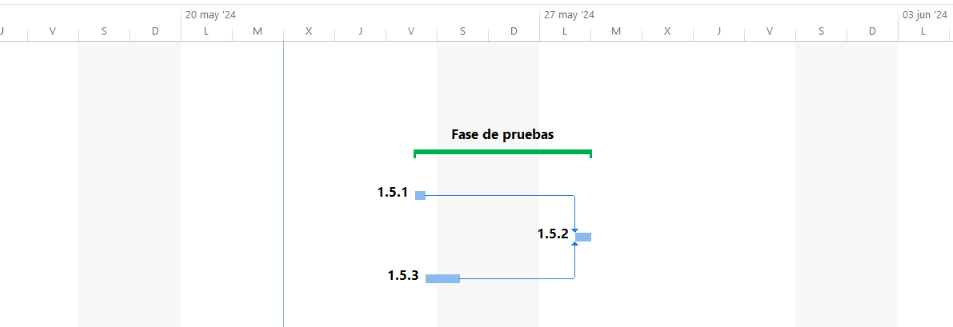
\includegraphics[width=1\linewidth]{figures/5-Gantt/5-Gantt-Pruebas.png}
    \caption{Planificación inicial. Diagrama de Gantt, fase de pruebas}
    \label{fig:5_PI-Gantt-Pruebas}
\end{figure}

\subsubsubsection{Planificación inicial. Despliegue del sistema}
En la \coloredUnderline{\hyperlink{table:5_PI-Despliegue}{\ref*{table:5_PI-Despliegue}: \nameref*{table:5_PI-Despliegue}}}, se detalla la planificación de las tareas que se deben realizar en la fase de despliegue del sistema.
El total de días estimados para la realización de esta fase es de 8 horas, desde el 12/06/2024 hasta el 13/06/2024.
\begin{table}[H]
    \centering
    \caption{Planificación inicial. Despliegue del sistema}
    \label{table:5_PI-Despliegue}
    \hypertarget{table:5_PI-Despliegue}{}
    \begin{tabular}{
       >{\columncolor{lightgreen!20}\raggedright\arraybackslash}p{1.5cm}
       >{\raggedright\arraybackslash}p{4.5cm}
       >{\raggedright\arraybackslash}p{2cm}
       >{\raggedright\arraybackslash}p{3cm}
       >{\raggedright\arraybackslash}p{3cm} }
    \rowcolor{darkgreen!50}
    \toprule
    \textbf{EDT} & \textbf{Nombre tarea} & \textbf{Duración} & \textbf{Fecha inicio} & \textbf{Fecha fin} \\
    \midrule
    1.6 & Despliegue del sistema & 8 horas & 12/06/2024 & 13/06/2024 \\
    \midrule
    1.6.1 & Configuración del servidor de Azure & 4 horas & 12/06/2024 & 12/06/2024 \\
    \midrule
    1.6.2 & Despliegue del \textit{frontend} & 4 horas & 12/06/2024 & 13/06/2024 \\
    \bottomrule
    \end{tabular}
\end{table}

En la \coloredUnderline{\hyperlink{fig:5_PI-Gantt-Despliegue}{Figura \ref*{fig:5_PI-Gantt-Despliegue}: \nameref*{fig:5_PI-Gantt-Despliegue}}}, se muestra el diagrama de Gantt de la planificación inicial de la fase de despliegue del sistema.
\begin{figure}[H]
    \hypertarget{fig:5_PI-Gantt-Despliegue}{}
    \centering
    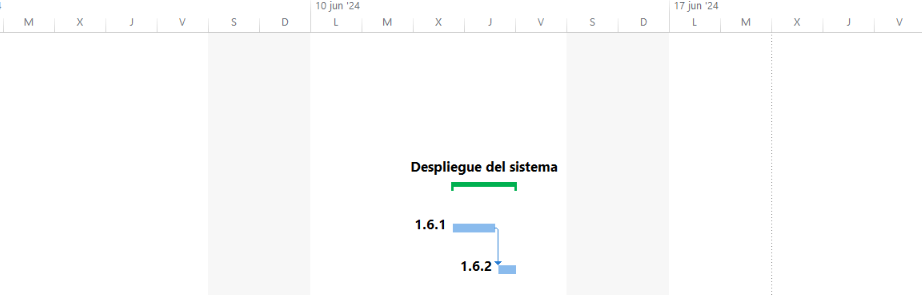
\includegraphics[width=1\linewidth]{figures/5-Gantt/5-Gantt-Despliegue.png}
    \caption{Planificación inicial. Diagrama de Gantt, despliegue del sistema}
    \label{fig:5_PI-Gantt-Despliegue}
\end{figure}

\subsubsubsection{Planificación inicial. Documentación del proyecto}
En la \coloredUnderline{\hyperlink{table:5_PI-Documentacion}{\ref*{table:5_PI-Documentacion}: \nameref*{table:5_PI-Documentacion}}}, se detalla la planificación de las tareas que se deben realizar en la fase de documentación del proyecto.
Esta fase se ha simplificado en el presente documento, de tal manera que para la tarea de la documentación de la memoria solo se especifica las tareas principales, sin detallar las subtareas.
\begin{longtable}{
    >{\columncolor{lightgreen!20}\raggedright\arraybackslash}p{1.5cm}
    >{\raggedright\arraybackslash}p{4.5cm}
    >{\raggedright\arraybackslash}p{2cm}
    >{\raggedright\arraybackslash}p{3cm}
    >{\raggedright\arraybackslash}p{3cm} }
    \caption{Cronograma del proyecto de documentación} \label{table:5_PI-Documentacion} 
    \hypertarget{table:5_PI-Documentacion}{}
    \\

    \toprule
    \rowcolor{darkgreen!50}
    \textbf{EDT} & \textbf{Nombre tarea} & \textbf{Duración} & \textbf{Fecha inicio} & \textbf{Fecha fin} \\
    \midrule
    \endfirsthead

    \toprule
    \rowcolor{darkgreen!50}
    \textbf{EDT} & \textbf{Nombre tarea} & \textbf{Duración} & \textbf{Fecha inicio} & \textbf{Fecha fin} \\
    \midrule
    \endhead

    \midrule
    \multicolumn{5}{r}{{Continúa en la siguiente página\ldots}} \\
    \endfoot

    \bottomrule
    \endlastfoot

    1.7 & Documentación del proyecto & 69.25 días & 02/04/2024 & 18/06/2024 \\
    \midrule
    1.7.1 & Creación de la plantilla en LaTeX & 4 horas & 01/06/2024 & 01/06/2024 \\
    \midrule
    1.7.2 & Redacción del documento final & 68.25 días & 02/04/2024 & 17/06/2024 \\
    \midrule
    1.7.2.1 & Introducción & 1 hora & 17/06/2024 & 17/06/2024 \\
    \midrule
    1.7.2.3 & Planificación del sistema de información & 9.38 días & 12/04/2024 & 22/04/2024 \\
    \midrule
    1.7.2.4& Definición de la arquitectura tecnológica & 16.75 días & 20/05/2024 & 08/06/2024 \\
    \midrule
    1.7.2.5 & Estudio de viabilidad del sistema & 2.13 días & 18/05/2024 & 20/05/2024 \\
    \midrule
    1.7.2.6 & Planificación y gestión del TFG & 44.69 días & 26/04/2024 & 15/06/2024 \\
    \midrule
    1.7.2.7 & Análisis del sistema de información & 58.69 días & 02/04/2024 & 07/06/2024 \\
    \midrule
    1.7.2.8 & Diseño del sistema de información & 11.13 días & 31/05/2024 & 12/06/2024 \\
    \midrule
    1.7.2.9 & Construcción del sistema de información & 12.88 días & 18/05/2024 & 01/06/2024 \\
    \midrule
    1.7.2.10 & Conclusiones y ampliaciones & 2 horas & 15/06/2024 & 15/06/2024 \\
    \midrule
    1.7.3 & Anexos & 20.81 días & 25/05/2024 & 17/06/2024 \\
    \midrule
    1.7.4 & Presentación proyecto & 4 horas & 18/06/2024 & 18/06/2024 \\
\end{longtable}

En la \coloredUnderline{\hyperlink{fig:5_PI-Gantt-Documentacion}{Figura \ref*{fig:5_PI-Gantt-Documentacion}: \nameref*{fig:5_PI-Gantt-Documentacion}}}, se muestra el diagrama de Gantt de la planificación inicial de la fase de documentación del proyecto.
\begin{figure}[H]
    \hypertarget{fig:5_PI-Gantt-Documentacion}{}
    \centering
    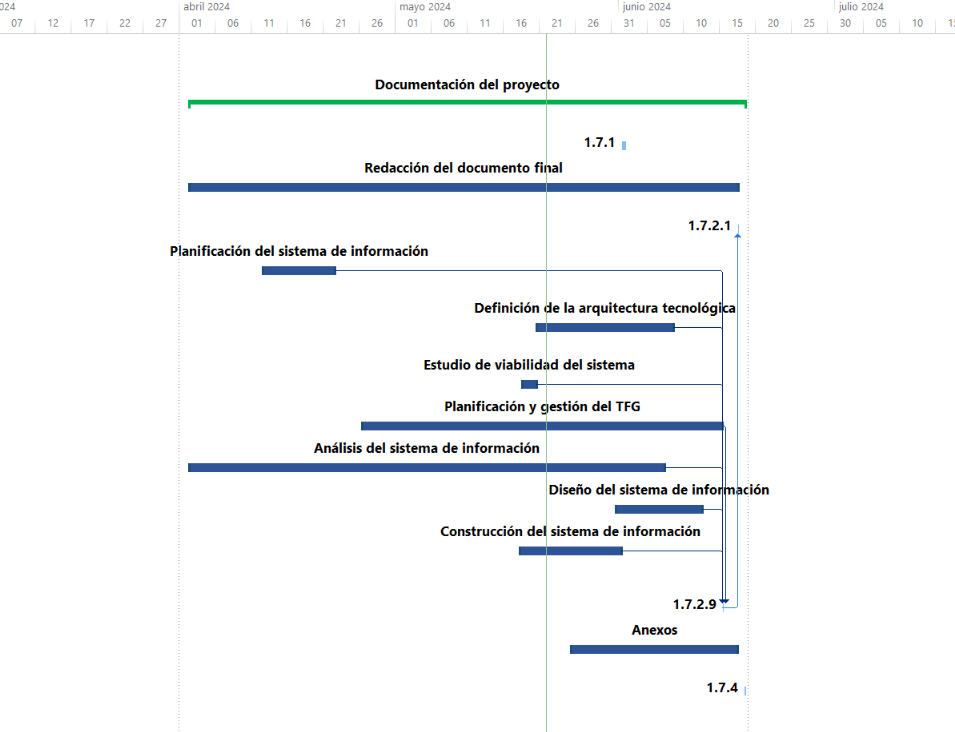
\includegraphics[width=1\linewidth]{figures/5-Gantt/5-Gantt-Documentacion.png}
    \caption{Planificación inicial. Diagrama de Gantt, documentación del proyecto}
    \label{fig:5_PI-Gantt-Documentacion}
\end{figure}